\documentclass[10pt,a4paper]{article}
\usepackage[utf8]{inputenc}
\usepackage{amsmath}
\usepackage{amsfonts}
\usepackage{amssymb}
\usepackage{graphicx}
\author{Andrea Colarieti Tosti}
\title{Rechenarchitektur Blatt 5 Lösung}

\begin{document}
\maketitle
\section{Aufgabe 23}
\subsection{a}
3+2 = 5 Bit
\subsection{b}
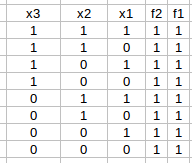
\includegraphics[scale=0.5]{tabelle1.png} \\
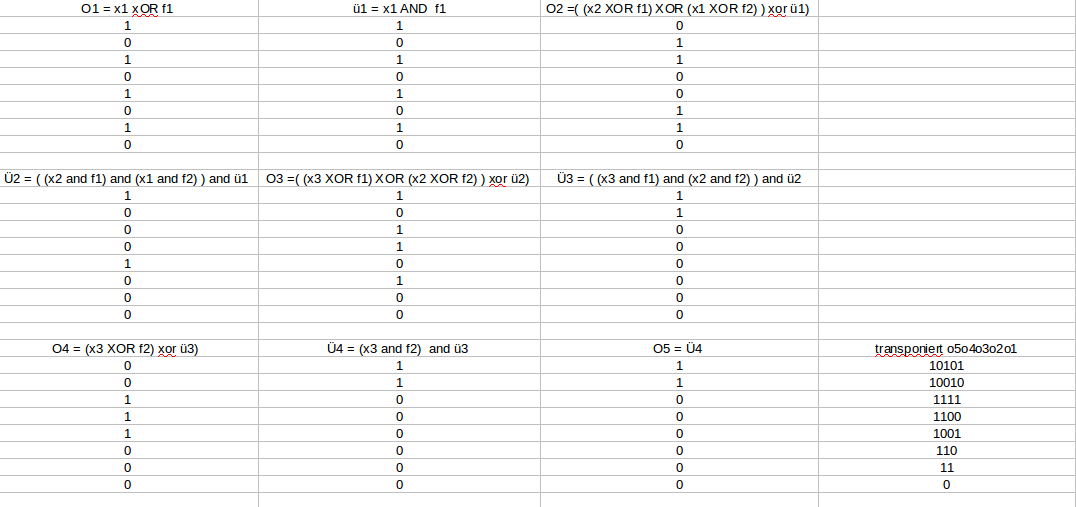
\includegraphics[scale=0.35]{tabelle2.png} 

\newpage
\subsection{c}
$o_1 = x_1 \oplus f_1$\\
Übertrag1= $ x_1 \wedge f_1 $\\\\
$o_2 = (x_2 \oplus f_1) \oplus (x_1 \oplus f_2) \oplus $Übertrag1 \\
Übertrag2=$o_2 = (x_2 \wedge f_1) \wedge (x_1 \wedge f_2) \wedge (x_1 \wedge f_1)$ \\\\
$o_2 = (x_3 \oplus f_1) \oplus (x_2 \oplus f_2) \oplus $Übertrag2  \\
Übertrag3= $(x_3 \wedge f_1) \wedge (x_2 \wedge f_2) \wedge $Übertrag2  \\\\
$o_3 = (x_4 \oplus f_1) \oplus (x_3 \oplus f_2) \oplus $Übertrag3  \\
Übertrag4= $(x_4 \wedge f_1) \wedge (x_3 \wedge f_2) \wedge $Übertrag3  \\\\
$o_4 = (x_5 \oplus f_1) \oplus (x_4 \oplus f_2) \oplus $Übertrag4\\
Übertrag= $(x_5 \wedge f_1) \wedge (x_4 \wedge f_2) \wedge $Übertrag5  \\\\
$o_5 = $Übertrag5\\\\
Zum vereinfachen müssen wir erst wissen, dass $a \oplus b = (\overline{a}\cdot b)+(a\cdot \overline{b})$.\\


\subsection{d}
Um eine dualzahl zu verdoppeln muss diese mal 2 gerechnet werden:\\
BinärZahl * 10 (Binär 2)\\
Alternativ könnten wir sagen, dass diese um eine stelle nach Links verschoben werden muss.

\section{Aufgabe 26}
a) : i\\
b) : ii\\
c) : iv\\
d) : ii\\
e) : iii\\
\end{document}